\documentclass[11pt, english]{scrartcl}

\usepackage[utf8]{inputenc}
\font\myfont=cmr11 at 60pt
\title{{\myfont Outlr\textcolor[HTML]{925FF0}{.}}}
\subtitle{A web application for analyzing \glspl*{subspace-outlier} on high dimensional datasets}
\author{Bennet Alexander Hörmann, Salomo Hummel,\\
Simeon Hendrik Schrape, Erik Bowen Wu, Udo Ian Zucker}

\usepackage{tabularx}
\usepackage{blindtext}
\usepackage{hyperref}
\usepackage[T1]{fontenc}
\usepackage[ddmmyyyy]{datetime} % must be after babel
\renewcommand{\dateseparator}{.}
\usepackage[margin=1.6in]{geometry} % Page margins
\usepackage{amsmath} % for $\text{}$
\usepackage[nameinlink]{cleveref}
\usepackage[section]{placeins}
\usepackage{xcolor}
\usepackage{svg}
\usepackage{graphicx}
\hypersetup{
	pdftitle={Software Requirements Specification},
    %linkbordercolor={red!10!gray},
    %urlbordercolor={red!10!gray},
    %citebordercolor={red!10!gray},
	colorlinks=true, % colored links instead of boxes
	%linkcolor={\textcolor[HTML]{045c5c}}, % dark blue
        %urlcolor={\textcolor[HTML]{045c5c}},
	%citecolor={\textcolor[HTML]{045c5c}},<
        allcolors = [HTML]{045c5c}
}
\usepackage{csquotes}
\usepackage{srs}
\usepackage[acronyms, toc]{glossaries}
\setlength{\parindent}{0pt}

% Glossary
\makeglossaries
\loadglsentries{glossaries}

\begin{document}
\maketitle
\pagebreak
\tableofcontents
\newpage

% INTRODUCTION ============================================================================

\section{Introduction}
With the recent rise in popularity of machine learning, research in outlier detection becomes more and more important since outliers degrade the performance of other machine learning methods. While the most effort is being put into improving general state-of-the-art methods, there are not many platforms allowing researchers to easily investigate \glspl{subspace-outlier} and the detection of these on high-dimensional data.\\
In \emph{Outlr.} we like to introduce a modern web service, which lets users run state-of-the-art \glspl{ODM} on specified sub-spaces of high-dimensional data sets and compare the results of the run while providing an accessible and intuitive user interface. Usually, this would require running many \glspl{experiment} manually on multiple \glspl{subspace}, which is hard to track.
With \emph{Outlr.} we aim to improve this workflow.\newline
The results are presented in an organized overview,
where the user can decide to further process them. Every user also has access to their previously run \glspl{experiment}, to avoid running the same \gls{experiment} more than once.
\newpage

% PRODUCT FUNCTIONS =======================================================================
\section{Product Functions}

% Mandatory product functions -------------------------------------------------------------
\subsection*{Mandatory product functions}

\productFunctionMust{User Management}{The application provides features to manage users. Users create accounts to store and access previously run \glspl{experiment}.}{crt:usr-management}

\productFunctionMust{Dashboard}{The dashboard gives users an intuitive overview of all the previous \glspl{experiment}.}{crt:dashboard}

\productFunctionMust{Create \gls{experiment}}{Users can create a new \gls{experiment} by entering the required data.}{crt:exp-create}

\productFunctionMust{Run \gls{experiment}}{After the user created an \gls{experiment} and selected all of the hyperparameters, the \gls{experiment} can be run that is to execute the \gls{ODM} on the given dataset.}{crt:exp-run}

\productFunctionMust{\Gls{experiment} results}{After an \gls{experiment} has been run the application provides detailed information about its result.}{crt:exp-result}

\pagebreak
% Optional product functions --------------------------------------------------------------
\subsection*{Optional product functions}

\productFunctionOptional{Landing page}{
The first page that users see is the landing page. On this page users can register or log in and when signed in log out. The page also informs potential users about the application.
}{crt:landing-page}

\productFunctionOptional{About us page}{The about us page gives users information about the developer team.
}{crt:about-us-page}

\productFunctionOptional{Compare \glspl{experiment}}{
This page shows diagrams that compare a selected set of \glspl{experiment}.
}{crt:compare-experiments}

\pagebreak

% REQUIREMENTS ============================================================================
\section{Requirements: Scope and Delimitation}

% Mandatory requirements ------------------------------------------------------------------
\subsection*{Mandatory requirements}

% Mandatory requirements: User management
\subsubsection*{User Management}
\mandatoryRequirement{Create account}{Users can create an account by providing a valid username and password.
\fulfills{crt:usr-management}
\fulfills{crt:landing-page}
}{usr-create}
\functional{usr-create}
\vspace{-\baselineskip}

\mandatoryRequirement{Login}{Users can log into their account by entering their usernames and their respective passwords. 
\fulfills{crt:usr-management}
\fulfills{crt:landing-page}
}{usr-login}
\functional{usr-login}


\mandatoryRequirement{Logout}{Users can log out of their account.
\fulfills{crt:usr-management}
\fulfills{crt:landing-page}
}{usr-logout}
\functional{usr-logout}

% Mandatory requirements: Dashboard
\subsubsection*{Dashboard}

\mandatoryRequirement{View dashboard}{
A dashboard provides an overview of all \glspl{experiment} that were run.
\fulfills{crt:dashboard}}{view-dashboard}
\functional{view-dashboard}

\mandatoryRequirement{Click on \gls{experiment} on dashboard}{
The dashboard entries are clickable and lead to the corresponding \gls{experiment} results.
\fulfills{crt:dashboard}}{dashboard-click}
\functional{dashboard-click}


\pagebreak
% Mandatory requirements: Create an experiment
\subsubsection*{Create \gls{experiment}}

\mandatoryRequirement{Name \glspl{experiment}}{
Users can name their \glspl{experiment}.
\fulfills{crt:exp-create}}{naming-experiment}
\functional{naming-experiment}

\mandatoryRequirement{Upload dataset as \gls{CSV} file}
{Users can upload a dataset as \gls{CSV} file.
\fulfills{crt:exp-create}}{ds-read}
\functional{ds-read}

\mandatoryRequirement{Upload \gls{ground-truth-file} as \gls{CSV} file}{Users can upload a \gls{ground-truth-file} when creating an \gls{experiment}.
\fulfills{crt:exp-create}}{gt-file}
\functional{gt-file}

%Users can select subspaces from the dataset for the subspace-logic
\mandatoryRequirement{Select subspaces from dataset}{Users can select subspaces from the dataset to be processed by the \gls{subspace-logic}.\fulfills{crt:exp-create}}{exp-create-select-subsets}
\functional{exp-create-select-subsets}

\mandatoryRequirement{Specify \gls{subspace-logic}}{Users can specify a \gls{subspace-logic} using \emph{logical or} and \emph{logical and} operators.\fulfills{crt:exp-create}}{exp-create-subspace-logic}
\functional{exp-create-subspace-logic}
\vspace{-\baselineskip}

\mandatoryRequirement{Customize hyperparameters}{
Based on the selected \gls{ODM} users can customize all its hyperparameters.
\fulfills{crt:exp-create}}{custom-param}
\functional{custom-param}

\mandatoryRequirement{Provide a significant number of \glspl{ODM}}
{Users can select an \gls{ODM} from a significant subset of the \glspl{ODM} provided by the \Gls{PyOD} library.\fulfills{crt:exp-create}}{odm-select}
\functional{odm-select}

% Mandatory requirements: Run experiment
\subsubsection*{Run \gls{experiment}}

\mandatoryRequirement{Run \gls{experiment}}
{After creating an \gls{experiment} users can run it.\fulfills{crt:exp-run}}{exp-run}
\functional{exp-run}

% Mandatory requirements: Experiment results
\subsubsection*{\Gls{experiment} results}

\mandatoryRequirement{Display \gls{experiment} results}{
The app provides an overview page for every executed \gls{experiment} which includes the following information:
\begin{itemize}
    \item \Gls{experiment} name
    \item \gls{ODM} used for \gls{experiment}
    \item Accuracy
    \item Execution date and time
    \item Time taken to run the \gls{experiment}
    \item Number of detected outliers
    \item The \glspl{index} of the detected outliers
\end{itemize}
\fulfills{crt:exp-result}}{experiment-summary}
\functional{experiment-summary}

\mandatoryRequirement{Download detected outliers}{Users can download the \glspl{index} of the detected outliers from an \gls{experiment} as a \gls{CSV} file.
\fulfills{crt:exp-result}}{download-outliers}
\functional{download-outliers}

\pagebreak
% Mandatory requirements: Others
\subsubsection*{Others}

\mandatoryRequirement{English language}{The language of the application is english.}{english-language}
\nonFunctional{english-language}

\mandatoryRequirement{User password is stored securely}{
User passwords are stored using hashing and other methods for security.
}{securely-store-password}
\nonFunctional{securely-store-password}

\mandatoryRequirement{Unexpected errors}{If an unexpected error occurs, the application will not crash and instead notify the user.}{unexpected-errors}
\nonFunctional{unexpected-errors}

\mandatoryRequirement{Good reliability and maturity}{
The application is reliable and mature, which is achieved by extensive testing throughout the project.
}{reliability-and-maturity}
\nonFunctional{reliability-and-maturity}

\mandatoryRequirement{Easy to learn and efficient workflows}{
For the target group (see \ref{section:target-group}), the application is easy to learn and provides efficient workflows.
}{usability-and-learnability}
\nonFunctional{usability-and-learnability}

\mandatoryRequirement{Good resource handling}{
The application releases all resources of an \gls{experiment} after it is run. Only the results that the user needs will be saved.
}{resource-handling}
\nonFunctional{resource-handling}

\mandatoryRequirement{Good maintainability}{
The source code of the application is easy to read and modify. This requires a good code structure and good documentation achieved by helpful comments.
}{maintainability}
\nonFunctional{maintainability}
\vspace{-\baselineskip}

\mandatoryRequirement{Modern and appealing \gls{GUI}}{
The \gls{GUI} of the application is designed to look modern and appealing. By default, the website has a dark theme.
}{modern-gui}
\nonFunctional{modern-gui}


\pagebreak
% Optional requirements -------------------------------------------------------------------
\subsection*{Optional requirements}

% Optional requirements: User management
\subsubsection*{User management}

\optionalRequirement{Delete account}{
Users can delete their account.
\fulfills{crt:usr-management}}{usr-delete-account}
\functional{usr-delete-account}

\optionalRequirement{Create user with email}{Users provide an email when creating an account. Afterward, they have to confirm their email by opening a verification link sent to their email.
\fulfills{crt:usr-management}}{usr-create-optional}
\functional{usr-create-optional}

\optionalRequirement{Login with email instead of username}{Users can also log into their account by entering their email and the respective password.
\fulfills{crt:usr-management}}{usr-login-optional}
\functional{usr-login-optional}

\optionalRequirement{Share \gls{experiment} result link}{
Users can create and share a link to an \gls{experiment} so that other users can see its results when opening the link.
\fulfills{crt:usr-management}}{usr-exp-share}
\functional{usr-exp-share}

\optionalRequirement{Users can try out functions}{
Users can try out the application without an account.
\fulfills{crt:usr-management}}{usr-without-account}
\functional{usr-without-account}

\optionalRequirement{Forgot password feature}{
When users forget their password they can set a new password after sufficient proof of identity.
\fulfills{crt:usr-management}}{use-forgot-passwd}
\functional{use-forgot-passwd}


\pagebreak
% Optional requirements: Dashboard
\subsubsection*{Dashboard}
\optionalRequirement{Filter and search \glspl{experiment} on dashboard}{
Users can filter and search the \glspl{experiment} shown on the dashboard.
\fulfills{crt:dashboard}
}{dashboard-filtered}
\functional{dashboard-filtered}

\optionalRequirement{Sort \glspl{experiment} on dashboard}{
Users can sort the \glspl{experiment} shown on the dashboard.
\fulfills{crt:dashboard}}{dashboard-sort}
\functional{dashboard-sort}

\optionalRequirement{Loading animations}{
The application shows a loading animation when it waits for the results of an \gls{experiment}.
\fulfills{crt:dashboard}
\fulfills{crt:exp-result}}{dashboard-loading-animations}
\functional{dashboard-loading-animations}

% Optional requirements: Create an experiment
\subsubsection*{Create \gls{experiment}}

\optionalRequirement{Upload \gls{CSV} file containing generated data}{
Users can upload a \gls{CSV} file containing generated data, which is merged with the uploaded dataset before running the \gls{experiment}.
\fulfills{crt:exp-create}}{upload-generated-data}
\functional{upload-generated-data}

\optionalRequirement{Create new \gls{experiment} based on a previously run \gls{experiment}}{
A new \gls{experiment} can be created by copying a previously run \gls{experiment}. Users only need to re-upload the dataset and \gls{ground-truth-file}.
\fulfills{crt:exp-create}}{copy-experiment}
\functional{copy-experiment}

\optionalRequirement{Name dataset}{
Users can specify a name for an uploaded dataset, which is displayed in \gls{experiment} results and the dashboard.
\fulfills{crt:dashboard}}{name-dataset}
\fulfills{crt:exp-create}
\fulfills{crt:exp-result}
\functional{name-dataset}


\optionalRequirement{\Gls{subspace-logic} can be nested}{
\Gls{subspace-logic} may contain nestings of logical operators.
\fulfills{crt:exp-create}}{exp-create-nested-subspace-logic}
\functional{exp-create-nested-subspace-logic}

\optionalRequirement{Find outliers in given number of \glspl{subspace}}{
Users can specify a list of \glspl{subspace} and a number $k$, so that the \gls{experiment} identifies all \glspl{datapoint}, that are outliers in at least $k$ of the given \glspl{subspace}.
\fulfills{crt:exp-create}}{exp-create-subspace-count}
\functional{exp-create-subspace-count}
\vspace{-\baselineskip}

\pagebreak

\optionalRequirement{Use column headers}{
A \gls{subspace} can be specified by naming the column headers of the columns that are included in the \gls{subspace}.
\fulfills{crt:exp-create}}{exp-create-column-headers}
\functional{exp-create-column-headers}

\optionalRequirement{Users can apply their own \gls{ODM}}{
Instead of selecting an \gls{ODM} from the list users can upload their own \gls{ODM}. \fulfills{crt:exp-create}}{apply-own-odm}
\functional{apply-own-odm}

\vspace{-\baselineskip}

\optionalRequirement{Provide all \glspl{ODM} from \gls{PyOD}}
{The app provides all \glspl{ODM} from \gls{PyOD}.
\fulfills{crt:exp-create}}{more-odm}
\functional{more-odm}

\optionalRequirement{No \gls{ground-truth-file} needed}{The user does not have to add a \gls{ground-truth-file} to the dataset. 
\fulfills{crt:exp-create}}{without-gt-file}
\functional{without-gt-file}

\optionalRequirement{Drag and drop support}{The user can drag and drop the \gls{CSV} files for the dataset and \gls{ground-truth-file}.
\fulfills{crt:exp-create}}{drag-drop}
\functional{drag-drop}

\optionalRequirement{Dataset preprocessing}{Users have options for preprocessing on the uploaded dataset.\fulfills{crt:exp-create}}{ds-preprocessing}
\functional{ds-preprocessing}

\optionalRequirement{Provide new \glspl{ODM}}{
The application provides \glspl{ODM} developed by our team.
\fulfills{crt:exp-run}}{exp-run-own-odm}
\functional{exp-run-own-odm}

\pagebreak
% Optional requirements: Run experiment
\subsubsection*{Run \gls{experiment}}

\optionalRequirement{Run \glspl{experiment} concurrently}{
The application runs \glspl{experiment} concurrently.
\fulfills{crt:exp-run}}{exp-run-concurrent}
\nonFunctional{exp-run-concurrent}

\optionalRequirement{Run \glspl{experiment} with \gls{hpp} range}{
Users can specify a range for a \gls{hpp} and a step size. When running the \gls{experiment}, the outlier detection is done for every step in the specified range. The application shows a diagram where the accuracy is plotted against the \gls{hpp} value.
\fulfills{crt:exp-run}}{exp-run-hyperparameter-range}
\functional{exp-run-hyperparameter-range}

% Optional requirements: Experiment results
\subsubsection*{\Gls{experiment} results}

\optionalRequirement{Show ROC curves}{
The application shows ROC curves for an \gls{experiment}.
\fulfills{crt:exp-result}}{roc-curve}
\functional{roc-curve}

\optionalRequirement{Display output log}{
The application displays output logs of the execution at the user's request.
\fulfills{crt:exp-result}}{output-log}
\functional{output-log}
\vspace{-\baselineskip}

% Optional requirements: Compare experiments
\optionalRequirement{Select \glspl{experiment} to compare}{
On the dashboard, users can select \glspl{experiment} to compare them.
\fulfills{crt:dashboard}\fulfills{crt:compare-experiments}}{dashboard-compare-experiments}
\functional{dashboard-compare-experiments}

\optionalRequirement{Compare \glspl{experiment}}{
The application shows diagrams that compare metrics from different \glspl{experiment} selected by the user. For example, the ROC curves can be displayed in a single graph or a histogram can be displayed to compare accuracies.
\fulfills{crt:compare-experiments}}{compare-experiments-page}
\functional{compare-experiments-page}


\subsubsection*{Others}

\optionalRequirement{Light theme}{
Users can change the \gls{GUI} to a light theme.
\fulfills{crt:usr-management}}{light-mode}
\nonFunctional{light-mode}


\pagebreak

\newpage
% Delimitation ----------------------------------------------------------------------------
\subsection*{Delimitation}

\delimitation{No mobile version}{d-mobile-ver} 
A mobile application is not planned.  \\

\delimitation{Application not optimized for mobile devices}{d-opt-mobile} 
Optimizing the website for mobile devices is not planned. \\

\delimitation{No guarantee regarding the provided \glspl{ODM} from \Gls{PyOD}}{d-no-odm-guarantees}
The application uses \Gls{PyOD} in the backend and thus the performance, correctness, and reliability of the provided \glspl{ODM} are only as good as \Gls{PyOD} implements them. \\

\delimitation{Usability for users unfamiliar with outlier detection}{d-no-new-user-friendly}
For users unfamiliar with outlier detection, the application may be confusing. However, we do not aim to improve this experience.

\pagebreak


% PRODUCT USE AND ENVIRONMENT =============================================================
\section{Product Use and Environment}

\subsection*{Target group} \label{section:target-group}
The target group are people interested in researching \glspl{subspace-outlier} since the application provides useful tools for analyzing outliers in different subspaces and comparing different \glspl{ODM} on these subspaces. The application makes it easy to run and organize many \glspl{experiment} using different ODMs and combinations of subspaces.

\subsection*{Operating conditions and environment}
The client-side application runs on any PC running Windows ($\geq 10$) or common Linux distributions. It also requires Firefox ($\geq 107.0$) or Chrome ($\geq 107.0$) and an internet connection.\\
The server-side application can be deployed to any common Linux server that is able to run a \gls{python} interpreter.
\pagebreak


% PRODUCT OVERVIEW ========================================================================
\section{Product Overview}

\paragraph{General application structure}
The following use-case diagram\footnote{To simplify the diagram, connections between the user and use-cases are omitted if a use-case extends another use-case that is already connected to the user.} shows the general application structure from the perspective of a user.

\begin{figure}[h!]
    \centering
    \includesvg[width=\textwidth]{image/product_overview/use_case_diagram.svg}
    \caption{\label{fig:use-case-diagram}General structure use-case diagram}
\end{figure}

\paragraph{Create and run \gls{experiment}}
The following activity diagram shows the process of creating and running \glspl{experiment}.

\begin{figure}[h!t]
    \centering
    \includesvg[width=\textwidth]{image/product_overview/activity_diagram.svg}
    \caption{\label{fig:activity-diagram}\Gls{experiment} activity diagram}
\end{figure}

\newpage

% PRODUCT DATA ============================================================================
\section{Product Data} 
\label{product-data}
\hypertarget{product-data}{}

\subsection*{User profile data}
\begin{itemize}
    \item Username
    \item Authentication data i.e. password hash
    \item List of all \glspl{experiment}
\end{itemize}

\subsection*{\Gls{experiment} data}
\begin{itemize}
    \item Name given by the user
    \item \Gls{ODM} used
    \item Hyperparameters
    \item Execution date
    \item Time taken for execution
    \item Number of outliers detected
    \item \Glspl{subspace} and \gls{subspace-logic}
    \item Indices of detected outliers
    \item Accuracy
\end{itemize}

\pagebreak

% SYSTEM ARCHITECTURE =====================================================================
\section{System Architecture}
The application is modeled as a 3-Tier architecture consisting of a data tier, application tier, and presentation tier.
The data tier and application tier run on the server. The presentation tier runs in the browser.
The data tier is a \gls{SQL} database storing all persistent data.\footnote{See section
\ref{product-data} on product data
for detailed information}. 
The presentation tier is a web-based UI.
The data tier and presentation tier do not directly communicate with each other. All communication is handled by the application tier by accessing the database and providing an API for the presentation tier. It also handles all business logic e.g. execute the ODMs, apply the specified \gls{subspace-logic}, etc.  


\vspace{50pt}


    \begin{figure}[!ht]
    \centering
    \includesvg[width=\textwidth]{image/system_architecture/system_architecture.svg}
    \caption{\label{fig:system-architecture}Basic overview of the system architecture: the \gls{SQL} database represents the data tier, the backend represents the application tier and the web frontend represents the presentation tier}
    \end{figure}

\pagebreak

% PRODUCT PERFORMANCE =====================================================================
\section{Product Performance}

\par The application can maintain 20 000 user accounts. The application can handle 200 users at the same time while satisfying the following minimum performance requirements:

\begin{table}
    \centering
    \begin{tabularx}{0.8\textwidth} { 
      | >{\raggedright\arraybackslash}X 
      | >{\raggedleft\arraybackslash}X | }
     \hline
     Button response time & 200ms \\
     \hline
     Page navigation  & 200ms  \\
    \hline
    Run \gls{experiment} & not defined (see \productFunctionLink{d-no-odm-guarantees}) \\
    \hline
    Create User & 5sec \\ 
    \hline
    Log in & 2sec \\
    \hline
    Log out & 2sec \\
    \hline
    \end{tabularx}
    \caption{\label{table:min-performance}Minimum performance requirements}
\end{table}


\pagebreak

\section{GUI mockups}
\par The following mockups give an idea of how the \Gls{GUI} of the application may look like. The actual \gls{GUI} may deviate from these mockups. They also contain some elements, that are part of optional requirements and are not guaranteed to be present in the application. The intention of this section is solely to highlight certain product functions and corresponding requirements.

\pagebreak

\uimockup{Landing page}{
    The landing page is the first page that users see.}{
    \begin{figure}[h!t]
    \centering
    \includesvg[width=\textwidth]{image/mockups/landing_page_not_logged_in.svg}
    \caption{\label{svg-landing-page}Landing page when the user has not logged in yet. Elements depicted: sign up button, navigation bar, login button, try out button (optional)}
    \end{figure}
    
    \begin{figure}[h!t]
    \centering
    \includesvg[width=\textwidth]{image/mockups/landing_page_logged_in.svg}
    \caption{\label{svg-landing-page-logged-in}Landing page when the user has logged in. Elements depicted: navigate to dashboard button, navigation bar, profile menu}
    \end{figure}
        
}{mockup-landing-page} 
\mockupsProductFunction{crt:usr-management}
\mockupsProductFunction{crt:landing-page}
\mockupsRequirement{usr-create}
\mockupsRequirement{usr-logout}
\mockupsRequirement{view-dashboard}

\pagebreak

\uimockup{User Management}{
    Users can register and log in using the following forms.}{

        \begin{figure}[h!t]
        \centering
        \begin{minipage}{0.5\textwidth}
          \centering
          \includesvg[width=0.85\linewidth]{image/mockups/login_unselected.svg}
          \captionof{figure}{Login form (unselected)}
          \label{svg-login-form-unselected}
        \end{minipage}%
        \begin{minipage}{0.5\textwidth}
          \centering
          \includesvg[width=0.85\linewidth]{image/mockups/register_unselected.svg}
          \captionof{figure}{Register form (unselected)}
          \label{svg-register-form-unselected}
        \end{minipage}
        \begin{minipage}{0.5\textwidth}
          \centering
          \includesvg[width=0.85\linewidth]{image/mockups/login.svg}
          \captionof{figure}{Login form}
          \label{svg-login-form}
        \end{minipage}%
        \begin{minipage}{0.5\textwidth}
          \centering
          \includesvg[width=0.85\linewidth]{image/mockups/register.svg}
          \captionof{figure}{Register form}
          \label{svg-register-form}
        \end{minipage}
        \end{figure}
    
    }{mockup-login-register}
    \mockupsProductFunction{crt:usr-management}
    \mockupsRequirement{usr-create}
    \mockupsRequirement{usr-login}
    \mockupsRequirement{usr-logout}
    \mockupsRequirement{usr-create-optional}

\newpage

\uimockup{Create \gls{experiment}}{
    Dedicated page allowing users to create a new \gls{experiment}.}{
    \begin{figure}[h!t]
    \centering
    \includesvg[width=\textwidth]{image/mockups/create_experiment.svg}
    \caption{\label{svg-create-experiment}Create \gls{experiment} page. Elements depicted: upload dataset, upload \gls{ground-truth-file}, dataset preview and summary, select \gls{ODM}, specify hyperparameters, \gls{subspace-logic}, \gls{experiment} name (optional), dataset name (optional), run \gls{experiment} button}
    \end{figure}
}{mockup-create-experiment}
\mockupsProductFunction{crt:exp-create}
\mockupsProductFunction{crt:exp-run}
\mockupsRequirement{ds-read}
\mockupsRequirement{gt-file}
\mockupsRequirement{exp-create-select-subsets}
\mockupsRequirement{custom-param}
\mockupsRequirement{odm-select}
\mockupsRequirement{exp-run}
    
\newpage
    
\uimockup{Dashboard}{
    The dashboard gives users an overview of the previous \glspl{experiment}. According to optional requirements, the user may choose to refresh, compare, search, delete \glspl{experiment}, clear, sort, and filter the dashboard.}{
    \begin{figure}[h!t]
    \centering
    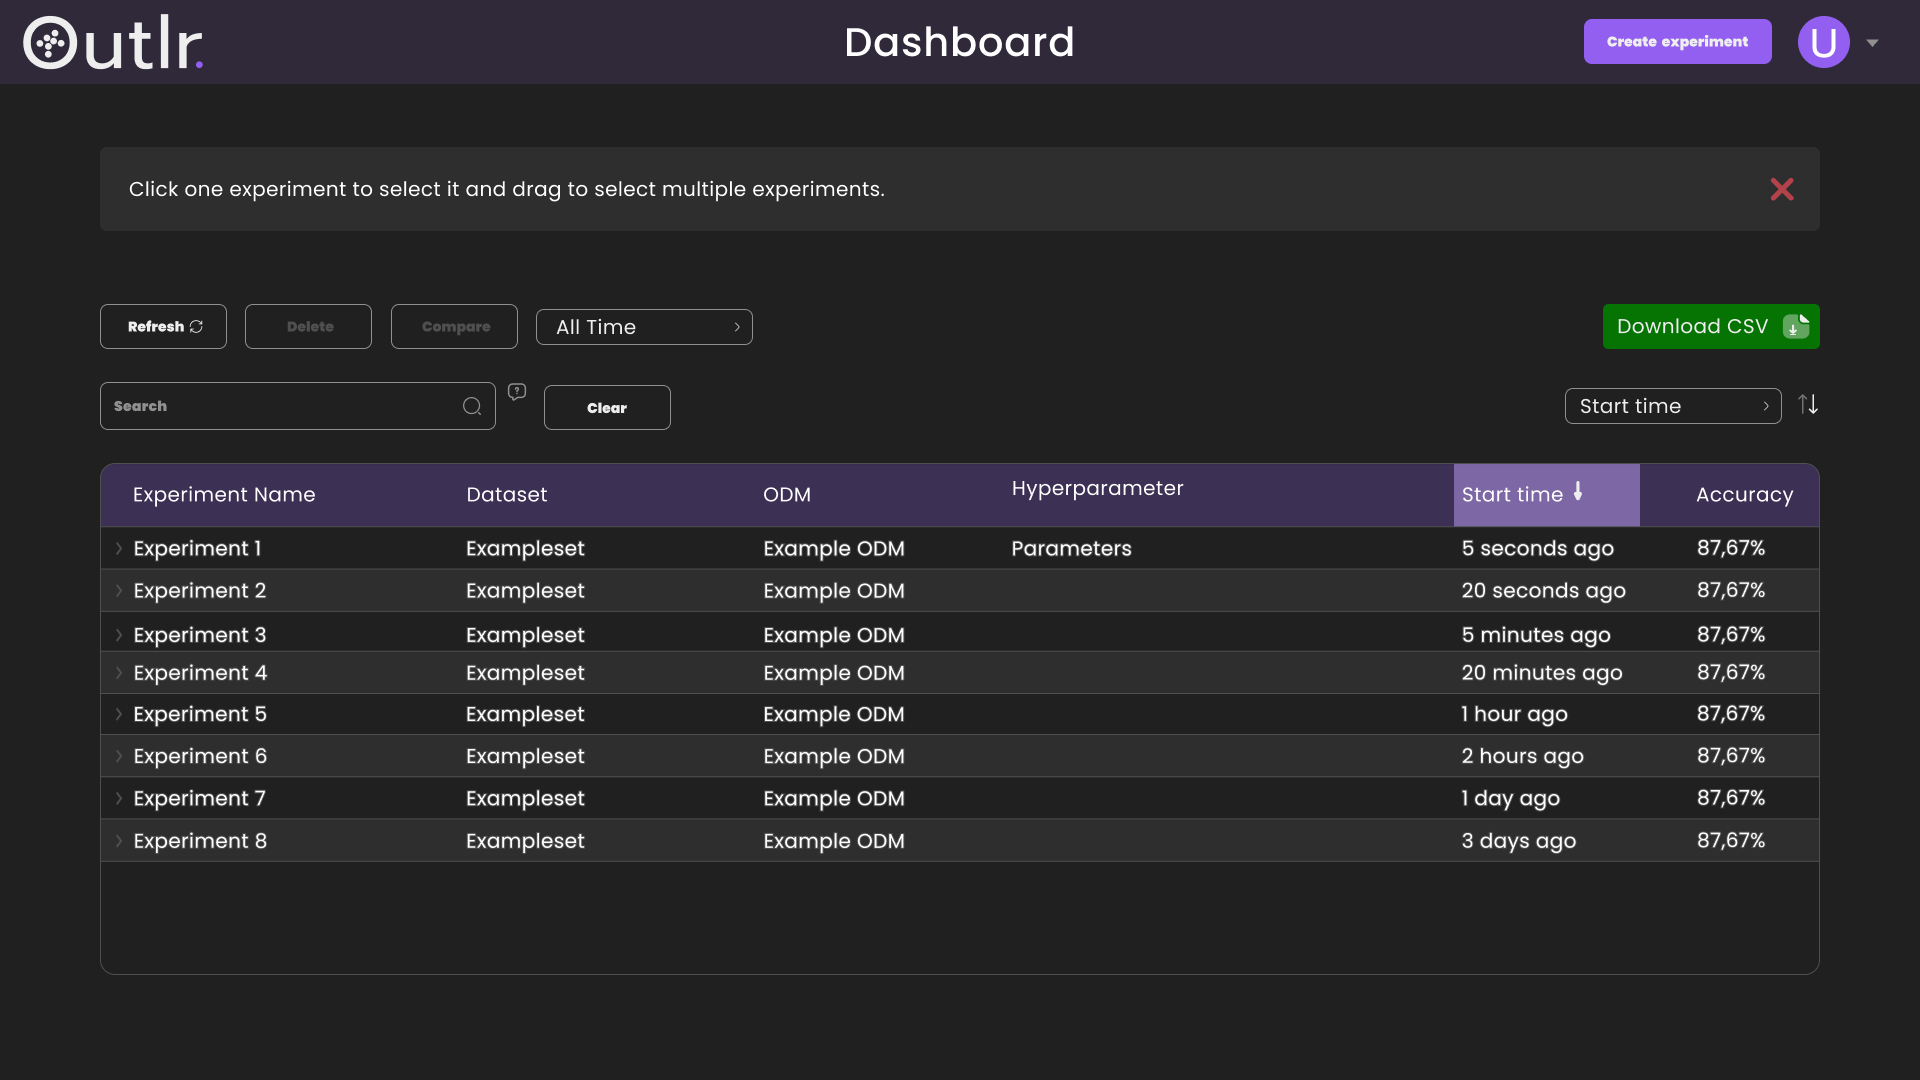
\includegraphics[width=\textwidth]{image/mockups/dashboard.png}
    \caption{\label{svg-dashboard}Dashboard. Elements depicted: table depicting previous \glspl{experiment}, hint box, download \gls{CSV} button, refresh, delete, compare, search and clear, time span filter, sorting type button and 
    create \gls{experiment} button} 
    \end{figure}
}{mockup-dashboard}
\mockupsProductFunction{crt:dashboard}
% \mockupsProductFunction{crt:usr-management}
\mockupsRequirement{usr-create}
\mockupsRequirement{usr-login}
\mockupsRequirement{usr-logout}

    \pagebreak

\uimockup{\Gls{experiment} result}{Dedicated page to display \gls{experiment} results.}{
    \begin{figure}[h!t]
    \centering
    \includesvg[width=\textwidth]{image/mockups/experiment_results.svg}
    \caption{\label{svg-experiment-result}\Gls{experiment} results. Elements depicted: \gls{experiment} summary, selected hyperparameters for \gls{ODM}, detected outliers and option to download them, roc curves  (optional)}
    \end{figure}
}{mockup-exp-result}
\mockupsProductFunction{crt:exp-result}
\mockupsRequirement{experiment-summary}
\mockupsRequirement{download-outliers}
\mockupsRequirement{roc-curve}

\pagebreak


% TESTCASES ===============================================================================
\section{Testcases}

% Testcases: User management --------------------------------------------------------------
\subsection*{User Management}

\testWithState{Create new account}{On signup window}{
    \tests{usr-create}
    \tests{usr-login}
    
    \teststepnostate{The user enters valid input and clicks on the signup button.}
        {Success message and entry in database}
    
    \teststepnostate
        {The user enters a username that already exists and clicks on the signup button.}
        {Error message and prompt to reenter credentials}}{tst:create-user}

\testWithState{Login}{On login window}{
    \tests {usr-login}
    
    \teststepnostate{The user enters valid input and clicks on the login button.}
        {Redirected to Dashboard}
        
    \teststepnostate{The user enters an incorrect password and clicks the login button.}
        {Error message, that password was entered incorrectly}
}{tst:login}

\test{Logout}{
    \tests {usr-logout}
    \teststepnostate{The user clicks the logout button.}
        {The user gets logged out.}
}{tst:logout}

\test{Download outliers as \gls{CSV} file}{
    \tests{download-outliers}

    \teststep{On \gls{experiment} results page}
        {The user clicks a button to download outliers.}
        {A \gls{CSV} file containing the \glspl{index} of all detected outliers is downloaded on the user's device.}

}{tst:download-outliers}

% Testcases: Dashboard --------------------------------------------------------------------
\subsection*{Dashboard}
\testWithState{Click \gls{experiment} from dashboard}{On dashboard}{
    \tests{view-dashboard}
    \tests{dashboard-click}
    
    \teststepnostate
        {The user clicks on an \gls{experiment} on the dashboard.}
        {The \gls{experiment} results of the selected \gls{experiment} are displayed to the user.}

    }{tst:dashboard-experiment-click}

% Testcases: Create experiment ------------------------------------------------------------
\subsection*{Create \gls{experiment}}

\testWithState{Upload \gls{CSV} files}{On create \gls{experiment} page}{
    \tests{ds-read}
    \tests{gt-file}
    
    \teststepnostate
    {User uploads a \gls{CSV} file that is not corrupted.}
    {The \gls{CSV} file is loaded to the server and its name is displayed on the create \gls{experiment} page.}

    \teststepnostate
    {User uploads a corrupted \gls{CSV} file.}
    {The \gls{CSV} file is not loaded to the server and an error message is displayed stating that the file cannot be read.}
    
}{tst:ds-read+gt-read}

\testWithState{\Gls{subspace} logic}
    {On create \gls{experiment} page}{
    
    \tests{exp-create-select-subsets}
    \tests{exp-create-subspace-logic}

    \teststepnostate
    {The user enters a correct textual expression describing the \gls{subspace-logic}.}
    {The \gls{subspace-logic} is saved and used once the \gls{experiment} starts running.}

    \teststepnostate
    {The user enters an incorrect textual expression for the \gls{subspace-logic}.}
    {An error message is displayed stating that the \gls{subspace-logic} expression could not be parsed.}
    
}{tst:sb-select+sb-logic}

\test{Select \gls{ODM} from dropdown menu}{
    \tests{odm-select}

    \teststep
    {On create \gls{experiment} page}
    {The user selects an \gls{ODM} from a dropdown menu.}
    {The correct \gls{ODM} is selected.}
    
}{tst:odm-selection}

\testWithState{Enter \glspl{hpp}}
    {On create \gls{experiment} page with already selected \gls{ODM}.}{
    \tests{custom-param}

    \teststepnostate
    {The user enters correct values for the \glspl{hpp}.}
    {The parameters are saved and used once the \gls{experiment} starts running.}
    
    \teststepnostate
    {The user enters incorrect values for the \glspl{hpp}.}
    {An error message is displayed stating which \glspl{hpp} are incorrect.}
    
}{tst:select-hyperparameters}

\pagebreak
\test{Try to run \gls{experiment} with missing inputs}{
    \tests{naming-experiment}
    \tests{ds-read}
    \tests{gt-file}
    \tests{exp-create-select-subsets}
    \tests{exp-create-subspace-logic}
    \tests{custom-param}
    \tests{odm-select}

    \teststep
    {On create \gls{experiment} page with some inputs incorrect or missing.}
    {The user tries to run the \gls{experiment}.}
    {The \gls{experiment} is not run and the incorrect and missing inputs are highlighted.}
    
}{tst:run-missing-inputs}


% Testcases: Run experiment ---------------------------------------------------------------
\subsection*{Run \gls{experiment}}

\test{Run \gls{experiment}}{
    \teststep
    {On create \gls{experiment} page with all required inputs entered correctly.}
    {The user clicks on a button to run the \gls{experiment}.}
    {The inserted data is fed to the selected \gls{ODM} which is run on the server.}
}{tst:run-exp}


% Testcases: Show experiment results ------------------------------------------------------
\subsection*{\Gls{experiment} results}
\testWithState{Display results of \gls{experiment} correctly}
    {An \gls{experiment} has been run successfully.}{
    \tests {experiment-summary}
    
    \teststepnostate{The user navigates to \gls{experiment} results}
    {The \gls{experiment} results are displayed correctly with no information missing.}

}{tst:experiment-results-after-successful-run}

\pagebreak

% DEVELOPER ENVIRONMENT ===================================================================
\section{Development environment}

\subsection*{Documents}
We used the following software to create the software requirements documentation, design documentation, and other documents:
\begin{itemize}
    \item \Gls{overleaf}
    \item \Gls{texlive} $\geq 2022$
\end{itemize}

\subsection*{Client side development}
We will be using the following software for client-side application development:
\begin{itemize}
    \item \Gls{typescript} $\geq 4.9$
    \item \Gls{HTML}
    \item \Gls{CSS}
    \item \Gls{vue-js} $\geq 3.2.45$
\end{itemize}
\subsection*{Server side development}
We will be using the following software for server-side application development:
\begin{itemize}
    \item \Gls{postgresql} $\geq 15$
    \item \Gls{python} $\geq 3.11.0$
    \item \Gls{pandas} $\geq 1.5.2$
    \item \Gls{PyOD} $\geq 1.0.6$
    \item \Gls{flask} $\geq 2.2.3$
\end{itemize}

\subsection*{Team organization}
For internal organization we will use the following tools:
\begin{itemize}
    \item \Gls{git} for version control
    \item \Gls{gitlab} for collaboration
\end{itemize}

\pagebreak

% GLOSSARIES ==============================================================================
\printglossary % print glossary
\pagebreak
\printglossary[type=\acronymtype] % print acronyms

\end{document}
